\todo{Introducera de tillämpningar som ska tagits upp; enkla primtal, tvillingsprimtal, primtal i aritmetiska talföljder, storleken på primtalsgap(?).}

%Over the course of this report we have refered to ,and approximated, the distribution of variouss classifications of prime numbers. Using now our implementation of Helfgott's origianl code we seeek to present the legitimacy of said distributions and also reflect on the quality of the code which we have written. The specific distributions ot be presented are those of the regula r prime numbers, the twin primes, as well as primes in arithmetic sequences. For each of these distributions have slight modifications been made to the code, which will be briefly discussed.

\subsubsection{Fördelningen av primtal}
\todo{Grafera antalet primtal vi har hittat jämfört emot PNT, både x/log x och Li(x). Diskutera sedan varför skillnader finns/ vad för slutsats vi kan dra(?)/ hur vi har kommit här?}
%Beginning with the classic example of the set of prime numbers, below is illustrated the distribution predicted by the familiar x over log x from sieve theory/Chebychev, the more accurate lorgarithmic integral Li(x), and the actual number of primes found in using our implementation. In order to generate the following graph, no new sieving methods were introduced, simply the counting fucntion in Appendix X
\begin{figure}[H]
    \centering
    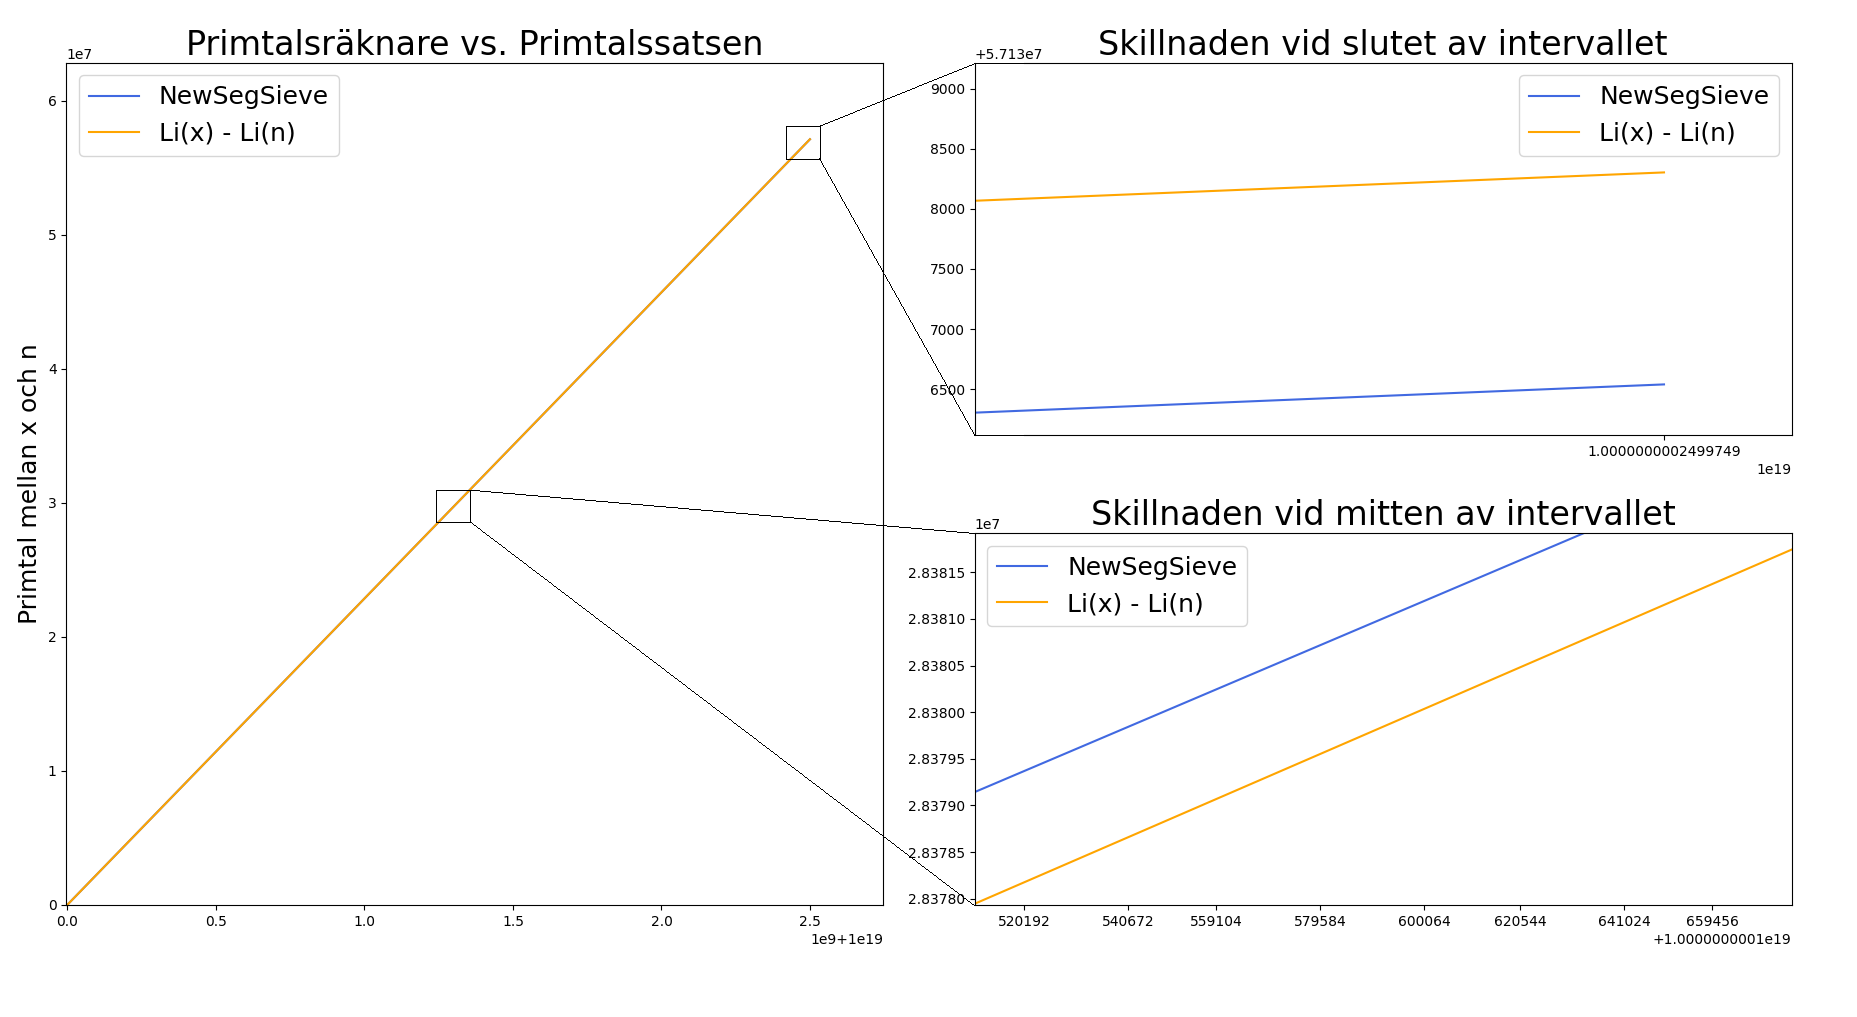
\includegraphics[width = \textwidth]{coen/Images/Primes.png}
    \caption{\todo{Infoga en graf med antalet primtal enligt koden, x/log x, och Li(x)}}
    %This graph shows the relative distributions of primees as per the aforementioned fucntions. Notice that while x over log x appears relatively close for smaller x the logarithmic integral approximation is a near exact match for the true distribution, so much so that the code line is hidden.
    \label{fig:res.prime}
\end{figure}
%As shown in figure X, should we believe in the PNT it seems as though our code does indeed find the correct number of primes. The rather large error in the x over log x estimate is indicative/reflective of one of the limitations highlighted in Section XXX, namely the impact of the error terms and their reconcillation with the main terms. Howeve, there doest exist a deeper link between the x over log x estimate and that of the logarithmic integral. Throguh the use of integral wizardry you can decompose the logarithmic integral into a series of terms, the first of which being x over log x with the remainder being of the order of sqrt(x). This then accounts for the increase in error as x grows. Thiese kinds of approximations for the prime counting function can also be rather naturally extrapolated to those for twin primes, as discussed below.

\subsubsection{Fördelningen av tvillingsprimtal}
\todo{Introducera de förändringarna som utfördes för att tillåta koden att sålla efter tvillingsprimtal.}
%Continuing our presentation of various sets of prime's distributions, next we turn to the other recurring theme of twin primes. The following figure illustrates the distributions of twin primes as predicted by x over log squared x and the second order logarithmic integral against those primes found using our implementation. It should be noted that a rather simple help function, Appendix XXX, was written which searches for non twin primes in the prime list and removes them.
\begin{figure}[H]
    \centering
    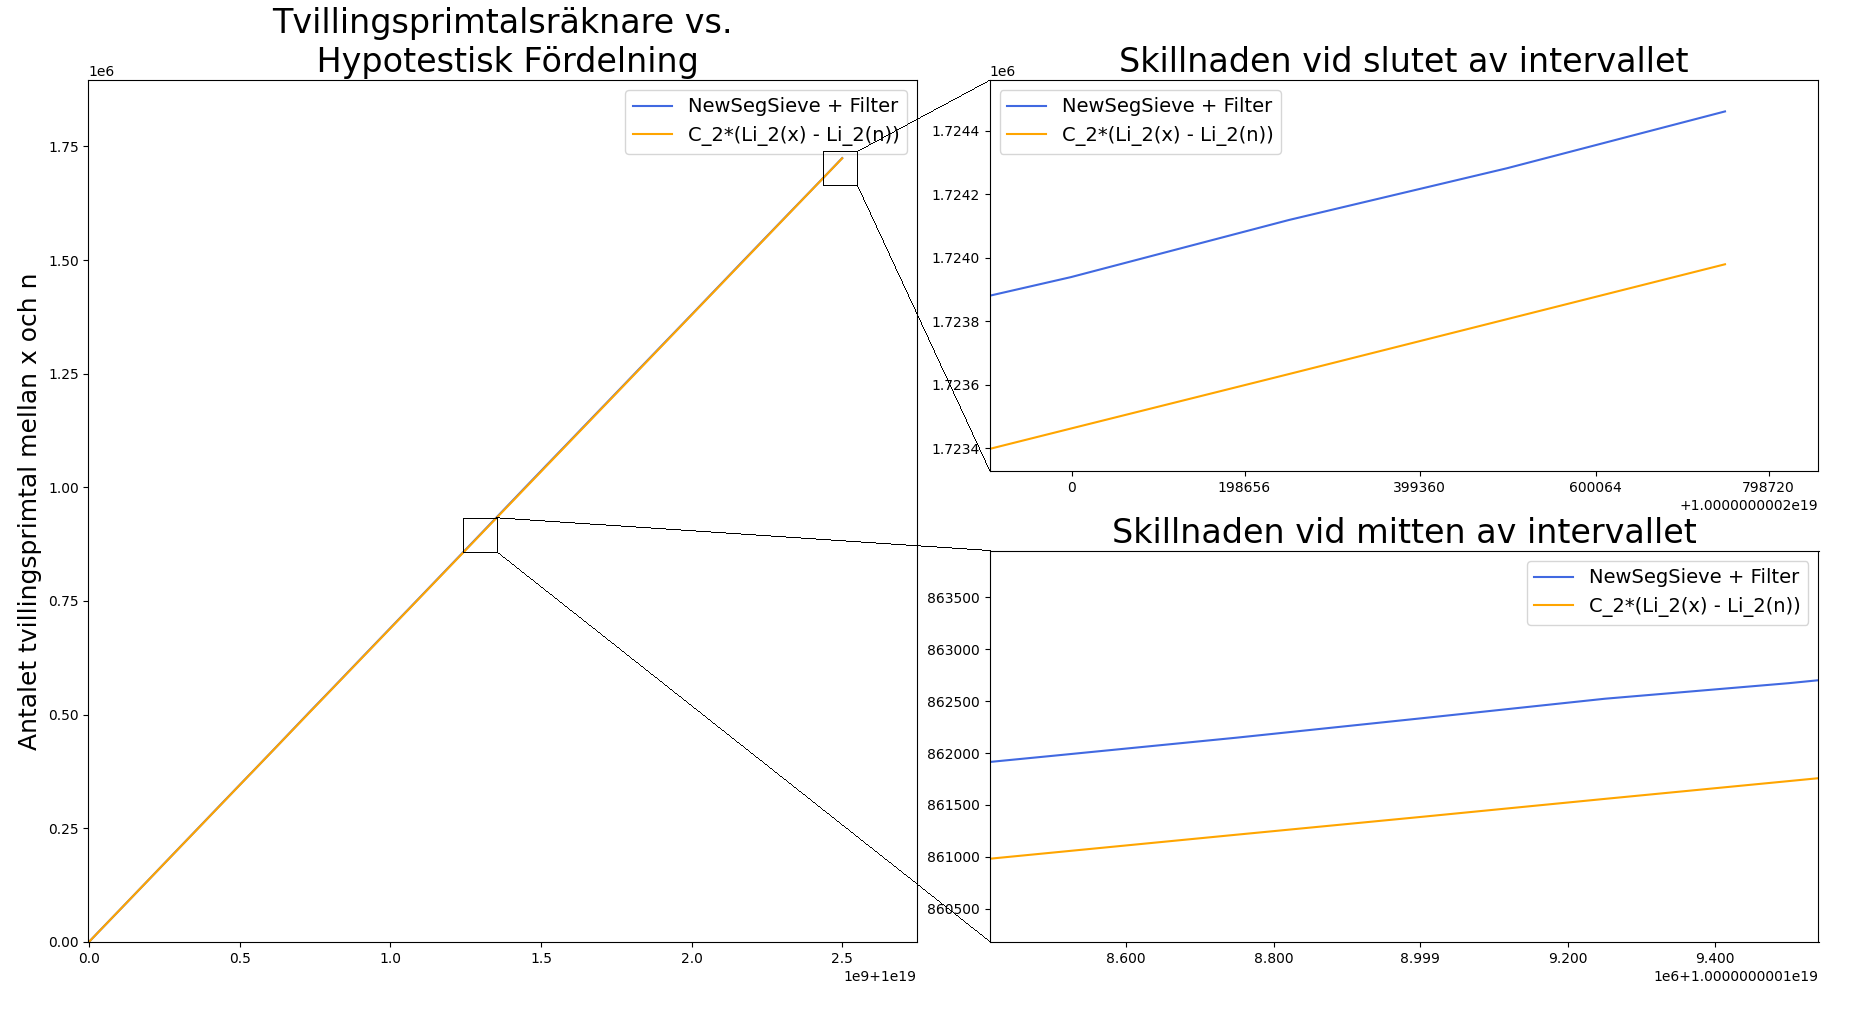
\includegraphics[width = \textwidth]{coen/Images/TwinPrimesNoKapp.png}
    \caption{\todo{Infoga en graf med antalet tvillingsprimtal enligt koden, Cx/log2 x, CLi\textunderscore2(x), undre begränsningen som finns i rapporten. Ge en motivation till varför C är vad det är och vartifrån fördelningen kommer.}}
    %This graph shows the relative distributions of the twin primes as per the aforementioned fucntions. Notice once again the accuarcy of the logarithmic integral, once again hiding our code line, as opposed to that of C x over log squared x, where the constant is 2*C_2, or 2 times the twin prime constant (discussed below).
    \label{fig:res.twins}
\end{figure}
\todo{Diskutera och förklara varför saker ser ut som de gör, vanliga saker. Kan vi lita på koden?(Kanske inte nödvändigt)}
%There are a number of things to discuss regardng the above figure. 
\subsubsection{Fördelningen av primtal i aritmetiska talföjlder}
\todo{Introducera de förändringarna som utfördes för att tillåta koden att sålla efter primtal i vissa aritmetiska talföljder.}
\begin{figure}[H]
    \centering
    
\includegraphics[width = 0.7\textwidth]{coen/Images/test.png}
    \caption{\todo{Infoga en graf med antalet primtal i aritmetiska följder enligt koden, Brun-Titchmarsh, Dirichlet serier(eller vad det nu var). Vad har vi valt epsilon till? Gör det något skillnad?}}
    \label{fig:res.arit}
\end{figure}
\todo{Diskutera ovanstående graf. Hur rimligt är uppskattningen? Hur dåligt är vår bästa approximation enligt koden?}